
%%%%%%%%%%%%%%%%%%%%%%%%%%%%%%%%%%%%%%%%%%%%%%%%%%%%%%%%%%%%%%
%%%%
\section{Bestimmung der Matrixelemente}
\label{sec:ME}

Um Gl.~\eqref{eq:k.p-H} l"osen zu k"onnen, ist es notwendig, die in ihr
vorkommenden Matrixelemente zu bestimmen. Eine wichtige Voraussetzung dazu
ist, da"s wir sowohl am $\Gamma$- als auch am L-Punkt eines Zinkblende-Gitters
die Wellenfunktionen reell w"ahlen k"onnen, wenn wir -- wie hier geschehen --
keine Spin-Bahn-Wechselwirkung ber"ucksichtigen. Dieser Effekt der
Zeitumkehrsymmetrie soll im folgenden kurz erl"autert werden.

Sei $\psi_{n\vec{k}}$ eine L"osung der station"aren Schr"odinger-Gleichung,
d.~h.\ 
%
\begin{displaymath}
    \op{H} \psi_{n\vec{k}} = \veps_{n}(\vec{k})\psi_{n\vec{k}},
\end{displaymath}
%
f"ur das Problem eines Teilchens in einem periodischen Potential. In diesem
Fall gilt das Bloch-Theorem
%
\begin{equation}
  \label{eq:Bloch-Theorem}
  \psi_{n\vec{k}}(\vec{r} + \vec{R}) = e^{i\sprod{k}{R}} \psi_{n\vec{k}}(\vec{r})
\end{equation}
%
f"ur alle Gittervektoren $\vec{R}$ des periodischen Potentials. Der
Wellenvektor \vec{k} h"angt also mit der diskreten Translationsinvarianz des
Problems zusammen. Ist \op{H} zeitumkehrinvariant, so ist aber auch
$\cc{\psi}_{n\vec{k}}$ ein L"osung der station"aren Schr"odinger-Gleichung zum
gleichen Eigenwert:\footnote{Betrachtet man die (zeitabh"angige)
  Schr"odinger-Gleichung, so sieht man, da"s die komplex-konjugierte Gleichung
  als zeitumgekehrte Gleichung aufgefa"st werden kann. F"ur einen
  zeitumkehrinvarianten Hamiltonoperator gilt also $\cc{\op{H}}=\op{H}$. Die
  Eigenwerte sind reell, da \op{H} hermitesch ist.}
%
\begin{displaymath}
  \op{H} \cc{\psi}_{n\vec{k}} = \veps_{n}(\vec{k}) \cc{\psi}_{n\vec{k}}
\end{displaymath}
%
Bilden wir nun das komplex-konjugierte von Gl.~\eqref{eq:Bloch-Theorem},
so erhalten wir
%
\begin{displaymath}
  \cc{\psi}_{n\vec{k}}(\vec{r} + \vec{R}) = e^{-i\sprod{k}{R}}
  \cc{\psi}_{n\vec{k}}(\vec{r}) ,
\end{displaymath}
%
d.~h.\ $\cc{\psi}_{n\vec{k}}$ geh"ort zum Wellenvektor \vec{-k}. Am
$\Gamma$-Punkt sind aber wegen $k=0$ sowohl $\psi_{n\vec{k}}$ als auch
$\cc{\psi}_{n\vec{k}}$ am gleichen Punkt im reziproken Raum angesiedelt.
F"ur den L-Punkt mit $\vec{k} = 2\pi/a_{\text{latt}} (1/2,1/2,1/2)$ gilt das
ebenso, da $-\vec{k} = \vec{k}- \vec{G}$ mit dem reziproken Gittervektor
$\vec{G} = 2\pi/a_{\text{latt}} (1,1,1)$ gilt, und somit
%
\begin{displaymath}
  \cc{\psi}_{n\vec{k}}(\vec{r} + \vec{R}) = 
  e^{-i\sprod{k}{R}} \cc{\psi}_{n\vec{k}}(\vec{r}) =
  e^{i\sprod{(k-G)}{R}} \cc{\psi}_{n\vec{k}}(\vec{r}) =
  e^{i\sprod{k}{R}} \cc{\psi}_{n\vec{k}}(\vec{r}),
\end{displaymath}
%
wegen $\sprod{G}{R}=2\pi n$ und $n \in \mathbb{Z}$ f"ur alle Gittervektoren
\vec{G} und \vec{R} des reziproken und realen Raumes. Wenn aber sowohl
$\psi_{n\vec{k}}$ als auch $\cc{\psi}_{n\vec{k}}$ Eigenzust"ande zum gleichen
Energie-Eigenwert und zum gleichen Wellenvektor sind, so k"onnen wir immer
reelle Funktionen $\frac{1}{2}(\psi_{n\vec{k}} + \cc{\psi}_{n\vec{k}})$ und
$\frac{1}{2i}(\psi_{n\vec{k}} - \cc{\psi}_{n\vec{k}})$ verwenden. Wir k"onnen
also davon ausgehen, da"s wir es in unserer Basis nur mit reellen
Wellenfunktionen zu tun haben. Dies bedeutet aber f"ur die in \op{H_{\Gamma
\text{L}}} [Gl.~\eqref{eq:k.p-H}] auftretenden Matrixelemente, da"s sie
ebenfalls reell sind. 


%%%%%%%%%%%%%%%%%%%%%%%%%%%%%%%%%%%%%%%%
\subsection{Betrag der Matrixelemente}
\label{sec:betrag}

F"ur $\V{11} = \V{35} = \V{15} = 0$ beschreibt Gl.~\eqref{eq:k.p-H}
den ungeordneten Kristall, den wir im Rahmen der TBA modellieren (siehe
Anhang~\ref{cha:lcao}). Damit k"onnen wir aber den Betrag der
Impulsmatrixelemente \PG\ und \PL\ sowie den Fernbandbeitrag $G$ aus den
effektiven Massen berechnen, die sich in der TBA-Rechnung ergeben. Dabei ist
die effektive Masse in der Umgebung von \vec{k_{\text{0}}} eigentlich ein
Tensor zweiter Stufe: 
%
\begin{displaymath}
%  \label{eq:m*-tensor}
   \frac{1}{m^{\ast}_{\alpha\beta}} = \left. \frac{1}{\hbar^{2}}
   \frac{\partial^{2} E}{\partial k_{\alpha} \partial k_{\beta}}
   \right|_{\vec{k}=\vec{k_{\text{0}}}} 
\end{displaymath}
%
F"ur die nichtentarteten Leitungsb"ander k"onnen wir diesen Tensor aber immer
auf Hauptachsenform bringen. Im Valenzband reichen am $\Gamma$-Punkt die
effektiven Massen in $[100]$-Richtung, am L-Punkt die in $[111]$- und $[1
\bar{1} 0]$-Richtung aus, um die Impulsmatrixelemente zu berechnen. Deshalb
k"onnen wir uns auf die zweite Ableitung bez"uglich der entsprechenden
Komponenten von \vec{k} beschr"anken.
%
\begin{equation}
  \label{eq:m*-d2E/dk2}
  \frac{1}{m^{\ast}} = \left. \frac{1}{\hbar^{2}} \frac{\partial^{2}
  E}{\partial k^{2}} \right|_{\vec{k}=\vec{k_{\text{0}}}}
\end{equation}
%
Die Energiedispersion $E(\vec{k})$ ist aber nicht analytisch bekannt. Vielmehr
mu"s der entsprechende TBA-Hamilton-Operator numerisch diagonalisiert 
werden. Wir k"onnen deshalb Gl.~\eqref{eq:m*-d2E/dk2} nicht direkt verwenden,
sondern m"ussen zu einer diskretisierten Form "ubergehen. Da das hier
verwendet Modell bez"uglich der Extrema \vec{k_{\text{0}}}
inversionssymmetrische Energiedispersionen liefert, erhalten wir
%
\begin{equation}
  \label{eq:m*-diskret}
  \frac{m}{m^{\ast}} = \frac{2m}{\hbar^{2}}
  \frac{E(\vec{k}) - E(\vec{k_{\text{0}}})}
  {(\vec{k} - \vec{k_{\text{0}}})^{2}}.
\end{equation}
%
Bei der Anwendung von Gl.~\eqref{eq:m*-diskret} mu"s sichergestellt werden,
da"s zum einen $\Delta k = |\vec{k}-\vec{k_{\text{0}}}|$ nicht zu gro"s wird,
da sonst die quadratische N"aherung der Dispersion nicht mehr gilt.
Andererseits darf $\Delta E = |E(\vec{k}) - E(\vec{k_{\text{0}}})|$ nicht zu
klein sein, da sonst Fehler in der Numerik
% und Unsicherheiten in den
%empirischen Parametern, die in den TBA-Hamilton-Operator eingehen, 
zu gro"ses
Gewicht erhalten. F"ur die Berechnung wurden typischerweise Werte von $\Delta E
= 0,2 \dots 4$~meV und $\Delta k = 0,001 \dots 0,04$ in Einheiten von
$2\pi/a_{\text{latt}}$ verwendet.

Damit erhalten wir die in Tab.~\ref{tab:Em*P} (siehe S.~\pageref{tab:Em*P})
dargestellten effektiven Massen.  Dabei ist zu beachten, da"s es sich bei
$m^{\text{v}}_{\Gamma}$ und $m^{\text{v}}_{\text{L}\perp}$ jeweils um die
Masse der leichten L"ocher handelt, die zu dem st"arker gekr"ummten Band
geh"ort (siehe auch Abb.~\ref{fig:band-long}). F"ur $m^{\text{c}}_{\Gamma}$
geben Emanuelsson \emph{et al.} \cite{edhm:94} einen Wert von
$(0,092\pm0,003)m$ an, in sehr guter "Ubereinstimmung mit unserem Ergebnis.

Aus der Beziehung
%
\begin{displaymath}
  \frac{m}{m^{\text{c}}_{\text{L}\parallel}} = 1 + \frac{2m}{\hbar^{2}}G
\end{displaymath}
%
ergibt sich der Fernbandbeitrag $G = -1,57$~eV\AA$^{2}$. Um \PG\ und \PL\ zu
bestimmen, diagonalisieren wir Gl.~\eqref{eq:k.p-H} f"ur $\V{11} = \V{35} =
\V{15} = 0$ in zweiter Ordnung St"orungstheorie, und erhalten die bekannten
Beziehungen 
%
\begin{subequations}
\label{eq:m*-P}
\begin{eqnarray}
  \label{eq:m*-PGC}
  \frac{m}{m^{\text{c}}_{\Gamma}} &=&
  1+ \frac{2m}{\hbar^{2}}\frac{|\PG|^{2}}{E_{\Gamma\text{c}}}\\
  \label{eq:m*-PGV}
  \frac{m}{m^{\text{v}}_{\Gamma}} &=&
  1- \frac{2m}{\hbar^{2}}\frac{|\PG|^{2}}{E_{\Gamma\text{c}}}\\
  \label{eq:m*-PLC}
  \frac{m}{m^{\text{c}}_{\text{L}\perp}} &=&
  1+ \frac{2m}{\hbar^{2}}\frac{|\PL|^{2}}{E_{\text{Lc}}-E_{\text{Lv}}}\\
  \label{eq:m*-PLV}
  \frac{m}{m^{\text{v}}_{\text{L}\perp}} &=& 1-
  \frac{2m}{\hbar^{2}}\frac{|\PL|^{2}}{E_{\text{Lc}}-E_{\text{Lv}}},
\end{eqnarray}
\end{subequations}
%
wobei wieder das Maximum des Valenzbandes als Nullpunkt der Energieskala
gew"ahlt wurde.  Um aus diesen Gleichungen \PG\ und \PL\ zu bestimmen,
ben"otigen wir noch die Energieeigenwerte der Niveaus, die sich in unserer
Basis befinden.  Tab.~\ref{tab:Em*P} zeigt die Ergebnisse, die wir mit Hilfe
der TBA erhalten haben. L"osen wir nun Gln.~\eqref{eq:m*-P} auf und setzen die
Energieeigenwerte und effektiven Massen aus Tab.~\ref{tab:Em*P} ein, so
erhalten wir die in der rechten Spalte von Tab.~\ref{tab:Em*P} aufgef"uhrten
Werte f"ur die Impulsmatrixelemente.
%
\begin{table}[bht]
%\setlength{\tabcolsep}{0.5ex}
\renewcommand{\arraystretch}{1.6}
  \begin{center}
    \begin{tabular}{c@{\hspace{2ex}}l@{\hspace{0.6ex}}r*{2}{@{\hspace{4ex}}l@{=\hspace{0.6ex}}r}}
%    \begin{tabular}{|c|l@{\hspace{0.6ex}}r|*{2}{l@{=\hspace{0.6ex}}r|}}
\hline\hline
Zustand 
& \multicolumn{2}{c}{\hspace{-4ex}Energie} 
& \multicolumn{2}{c}{\hspace{-4ex}effektive Masse}
& \multicolumn{2}{c}{Matrixelement}\\
\hline
\GCB 
& $E_{\Gamma\text{c}} =$ & 2,024 eV 
& $m^{\text{c}}_{\Gamma}$ & 0,0899 $m$
& $|\PG|$ & 8,83 eV\AA\\[1ex]
%\hline
\GVB
& $E_{\Gamma\text{v}} =$ & 0 eV
& $m^{\text{v}}_{\Gamma}$ & -- 0,0994 $m$
& $|\PG|$ & 9,24 eV\AA\\[1ex]
%\hline
 & \multicolumn{2}{l}{}
& $m^{\text{c}}_{\text{L}\perp}$ & 0,1349 $m$
& $|\PL|$ & 8,88 eV\AA\\
%\cline{4-7}
\raisebox{2.4ex}[-2,4ex]{\LCB}
& \raisebox{2.4ex}[-2,4ex]{$E_{\text{Lc}} =$} 
& \raisebox{2.4ex}[-2,4ex]{2,250 eV}
& $m^{\text{c}}_{\text{L}\parallel}$ & 1,699 $m$
& $G$ & -- 1,57 eV\AA$^{2}$\\[1ex]
%\hline
 & \multicolumn{2}{l}{}
& $m^{\text{v}}_{\text{L}\perp}$ & -- 0,1349 $m$
& $|\PL|$ & 10,2 eV\AA\\
%\cline{4-7}
\raisebox{2.4ex}[-2.4ex]{\LVB}
& \raisebox{2.4ex}[-2.4ex]{$E_{\text{Lv}} =$} 
& \raisebox{2.4ex}[-2.4ex]{-- 0,978 eV}
&  $m^{\text{v}}_{\text{L}\parallel}$ & 2,088 $m$
& \multicolumn{2}{l}{} \\[0.5ex]
\hline \hline
    \end{tabular}
    \caption{Energie, effektive Masse und daraus bestimmtes
      Impulsmatrixelement bzw. Fernbandbeitrag f"ur die Zust"ande \GCB, \GVB,
      \LCB\ und \LVB\ in ungeordnetem \GaInP.}
    \label{tab:Em*P}
  \end{center}
\renewcommand{\arraystretch}{0.625}
\end{table}
%

Es f"allt auf, da"s unser Modell keine einheitlichen Werte f"ur die
Impulsmatrixelemente liefert. Doch lassen sich diese Unterschiede zwanglos
durch die vernachl"assigten Fernbandbeitr"age erkl"aren. Da unser
Hauptaugenmerk den Zust"anden im Leitungsband gilt, wollen wir nur die Werte
verwenden, die sich aus den effektiven Massen im Leitungsband
ergeben. Weiterhin ist auff"allig, da"s sich die damit ergebenden Werte f"ur
\PG\ und \PL\ kaum unterscheiden. Darauf hatte schon Cardona \cite{card:63}
hingewiesen, und wir wollen deshalb im weiteren
%
\begin{displaymath}
  |\PG| = |\PL| = 8.86\text{~eV\AA}
\end{displaymath}
%
verwenden.

Bei der Bestimmung der Betr"age der Potentialmatrixelemente $\V{11}$, $\V{35}$
und $\V{15}$ gehen wir ganz "ahnlich vor. Zun"achst diagonalisieren wir
Gl.~\eqref{eq:k.p-H} f"ur $k=0$ in zweiter Ordnung St"orungstheorie.
Damit erhalten wir Ausdr"ucke f"ur die Kristallfeldaufspaltung
$\Delta_{\text{CF}}$, die Bandl"uckenreduzierung $\Delta E_{\text{BGR}}$ und
die "Anderung $\Delta E_{\Gamma \rightarrow \text{L}}$ der "Ubergangsenergie
$\bGVB{3}(\GVB) \rightarrow \bGCB (\LCB)$ in Abh"angigkeit von diesen drei
Matrixelementen:
%
\begin{subequations}
\label{eq:Delta-V}
\begin{eqnarray}
  \label{eq:DeltaCF}
  \Delta_{\text{CF}} &=&
  - \frac{|\V{35}|^{2}}{E_{\text{Lv}}} + \frac{|\V{15}|^{2}}{E_{\text{Lc}}} \\
  \label{eq:DeltaEBGR}
  \Delta E_{\text{BGR}} &=&
  \frac{|\V{11}|^{2}}{E_{\text{Lc}}-E_{\Gamma\text{c}}} -
  \frac{|\V{35}|^{2}}{E_{\text{Lv}}} \\
  \label{eq:DeltaEG-L}
  \Delta E_{\Gamma \rightarrow \text{L}} &=&
  \frac{|\V{11}|^{2}}{E_{\text{Lc}}-E_{\Gamma\text{c}}} +
  \frac{|\V{15}|^{2}}{E_{\text{Lc}}} + \frac{|\V{35}|^{2}}{E_{\text{Lv}}}
\end{eqnarray}
\end{subequations}
%
Wie bereits in Kap.~\ref{sec:materialsystem} erw"ahnt, sind die Gr"o"sen
$\theta = \Delta E_{\Gamma \rightarrow \text{L}} / \Delta E_{\text{BGR}}$ und
$\zeta = \Delta E_{\text{BGR}} / \Delta_{\text{CF}}$ aus theoretischen und
experimentellen Untersuchungen bekannt. Damit sind wir in der Lage, die
Potentialmatrixelemente \V{15} und \V{35} durch \V{11}, $\theta$ und $\zeta$
auszudr"ucken:
%
\begin{subequations}
\label{eq:V-V}
\begin{eqnarray}
  \label{eq:V35-V11}
  \frac{|\V{35}|^{2}}{E_{\text{Lv}}} &=& \frac{\theta - 1 -
    \frac{1}{\zeta}}{\theta + 2 - \frac{1}{\zeta}}
  \frac{|\V{11}|^{2}}{E_{\text{Lc}}-E_{\Gamma\text{c}}} =
  - 0.426 \frac{|\V{11}|^{2}}{E_{\text{Lc}}-E_{\Gamma\text{c}}} \\
  \label{eq:V15-V11}
  \frac{|\V{15}|^{2}}{E_{\text{Lc}}} &=& \frac{\theta - 1 +
    \frac{2}{\zeta}}{\theta + 2 - \frac{1}{\zeta}}
  \frac{|\V{11}|^{2}}{E_{\text{Lc}}-E_{\Gamma\text{c}}} = \;\;\: 0.110
  \frac{|\V{11}|^{2}}{E_{\text{Lc}}-E_{\Gamma\text{c}}}
\end{eqnarray}
\end{subequations}
%
Dabei haben wir die Werte der Gln.~\eqref{eq:zeta} und \eqref{eq:theta}
eingesetzt. 

Damit haben wir als einzigen freien Parameter das Matrixelement \V{11}, das in
unserem Modell den Grad der Ordnung beschreibt. Denn je gr"o"ser der
Ordnungsgrad ist, desto st"arker ist das Ordnungspotential, so da"s auch
\V{11} betragsm"a"sig gr"o"ser wird. Modellieren wir das Ordnungspotential
"uber VCA, so ist dieses proportional zum Ordnungsgrad $\eta$ \cite{rats:94},
und damit sind nat"urlich auch die Matrixelemente proportional zum
Ordnungsrad. Dies seinerseits f"uhrt dann zu konstanten Verh"altnissen
zwischen den Potentialmatrixelementen, die unabh"angig vom Ordnungsgrad sind,
wie in Gln.~\eqref{eq:V-V}.
%\marginpar{Etwas
%  "uber Vertrauensbereich wegen s. Ord. PT, Exp. eh nur f"ur geringe Ordnung
%  \dots}


%%%%%%%%%%%%%%%%%%%%%%%%%%%%%%%%%%%%%%%%
\subsection{Phase der Matrixelemente}
\label{sec:phase}

Als letzte unbekannte Gr"o"sen in unserem Modell, m"ussen wir nun noch die
Phasen der Matrixelemente bestimmen. Es reicht dabei aus die relativen
Vorzeichen zu bestimmen, da eine gemeinsame Phase aller Matrixelemente keine
Auswirkungen auf das Ergebnis hat, und aus dem oben gezeigten folgt, da"s die
Wellenfunktionen in unserer Basis, und damit auch die Matrixelemente, reell
w"ahlbar sind.  F"ur die Potentialmatrixelemente ist dies leicht zu sehen, da
\op{H_{1}(\vec{r})} eine reelle Funktion sein mu"s. Somit sind die
Potentialmatrixelemente Integrale "uber ein Produkt reeller Funtionen und
somit auch reell. Schreiben wir den Impulsoperator in Ortsdarstellung, so
erhalten wir f"ur die Impulsmatrixelemente ein Integral "uber das Produkt
einer reellen Funktion mit der Ableitung einer reellen Funktion, was wiederum
reell ist.
%
%\begin{displaymath}
%  \label{eq:PG-Ort}
%  \PG = - i \frac{\hbar}{m} \matrixel{\GCB}{\op{p_{x}}}{\GVBx} 
%      = \frac{\hbar^{2}}{m} \matrixel{\GVBx}{\pdx{x}}{\GCB},
%\end{displaymath}
%

Das Vorzeichen von \PG\ und \PL\ h"angt von der Wahl der Phasen der Zust"ande
ab. Um diese zu bestimmen, folgen wir dem Ansatz in Ref.~\cite{ccf:88}. Aus
einer TBA-Rechnung mit einer Basis aus einem $s$-artigen und drei
$p$-artigen Wellenfunktionen pro Atom erhalten wir ein schematisches Bild der
Wellenfunktionen in unserer Basis (siehe Anhang \ref{cha:lcao}). Diese Wellenfunktionen sind in
Abb.~\ref{fig:wfkt-G} f"ur den $\Gamma$-Punkt und in Abb.~\ref{fig:wfkt-L}
f"ur den L-Punkt skizziert. Grau schattierte Bereiche geben dabei ein positives
Vorzeichen der Wellenfunktion an, wei"se Bereiche bedeuten ein negatives
Vorzeichen. Im Bild zu \GCB\ sind zus"atzlich noch die Atome gekennzeichnet.
A1 und C1 bezeichnet Anion und Kation f"ur das Zinkblende-Gitter. A2 und C2
bezeichnet die Atome, die beim "Ubergang zur \CuPt-Einheitszelle dazukommen.
Skizzieren wir nun grob die Bereiche negativer \emph{Ableitung} bez"uglich $x$
der Leitungsband-Wellenfunktionen \GCB\ und \LCB, so stellen wir fest, da"s
die Verteilung der Vorzeichen im wesentlichen der der Valenzbandzust"ande
\GVBx\ und \LVBx\ entspricht. Das bedeutet aber, da"s das Produkt aus
Valenzband-Wellenfunktion und Ableitung der Leitungsbandwellenfunktion im
wesentlichen positiv ist, und somit auch die beiden Impulsmatrixelemente f"ur
\emph{diese} Wahl der Phasen positiv sind. Somit erhalten wir:
%
\begin{displaymath}
%  \label{eq:PG=PL}
  \PG = \PL = 8.86\text{~eV\AA}
\end{displaymath}
%
 
%\begin{sidewaysfigure}
\begin{figure}
  \centering
  \includegraphics[width=10cm]{G1c.eps}\raisebox{4cm}{(a)}
  \vspace{2ex}
  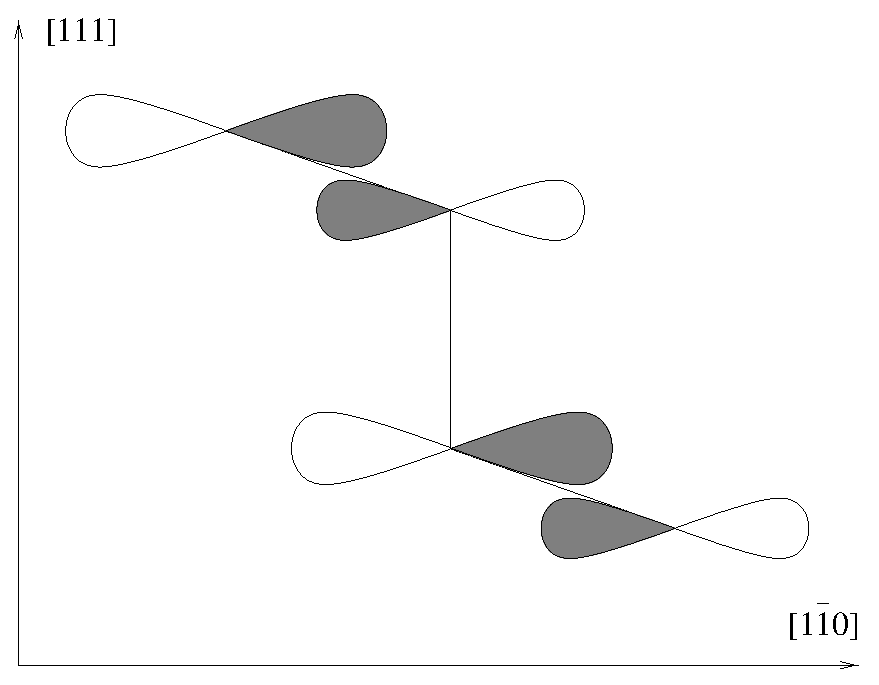
\includegraphics[width=10cm]{G5v.x.eps}\raisebox{4cm}{(b)}
  \caption{Schematische Darstellung der Wellenfunktionen von (a) \GCB\ und (b)
  \GVBx. $[1 \bar 1 0]$ entspricht der $x$-Richtung, $[111]$ der 
  $z$-Richtung. }
  \label{fig:wfkt-G}
\end{figure}
%\end{sidewaysfigure}

%\begin{sidewaysfigure}
\begin{figure}
  \centering
  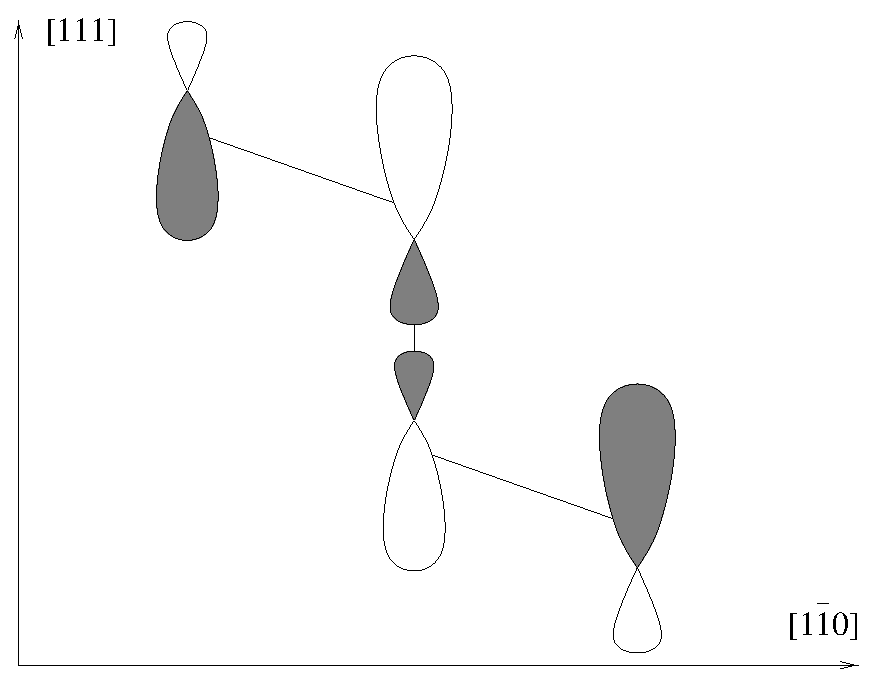
\includegraphics[width=10cm]{L1c.eps}\raisebox{4cm}{(a)}
  \vspace{2ex}
  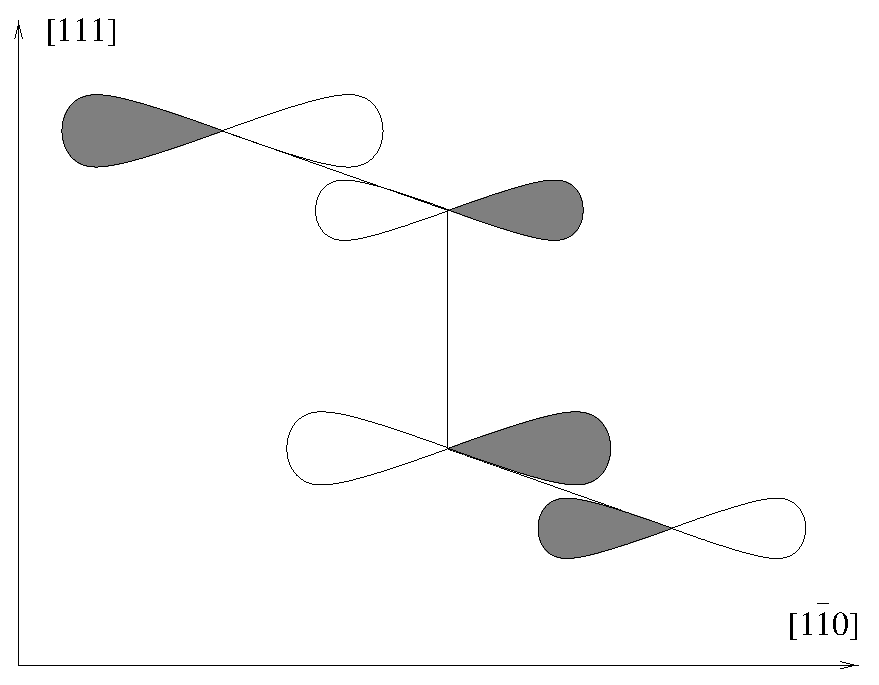
\includegraphics[width=10cm]{L3v.x.eps}\raisebox{4cm}{(b)}
  \caption{Schematische Darstellung der Wellenfunktionen von (a) \LCB\ und (b)
  \LVBx. $[1 \bar 1 0]$ entspricht der $x$-Richtung, $[111]$ der
  $z$-Richtung.}
  \label{fig:wfkt-L}
\end{figure}
%\end{sidewaysfigure}

Dadurch, da"s wir uns nun auf bestimmte Phasen der Wellenfunktionen in unserer
Basis festgelegt haben, sind im Prinzip auch die Vorzeichen der
Potentialmatrixelemente festgelegt. Doch treten dabei Schwierigkeiten auf, die
wir am Beispiel das Matrixelementes \V{35} illustrieren wollen. 

Die in Abb.~\ref{fig:wfkt-G}(b) und Abb.~\ref{fig:wfkt-L}(b) skizzierten
Valenzband-Wellenfunk"-ti"-onen lassen sich in der \CuPt-Einheitszelle als
%
\begin{subequations}
\label{eq:wfkt-tba}
\begin{eqnarray}
  \label{eq:G5v-tba}
  \ket{\GVBx} &=& -\alpha_{\Gamma} (\ket{x_{c1}} + \ket{x_{c2}})
  + \beta_{\Gamma} (\ket{x_{a1}} + \ket{x_{a2}}) \\
  \label{eq:L3v-tba}
  \ket{\LVBx} &=& +\alpha_{\text{L}} (\ket{x_{c1}} - \ket{x_{c2}}) +
  \beta_{\text{L}} (\ket{x_{a1}} - \ket{x_{a2}})
\end{eqnarray}
\end{subequations}
%
schreiben. Dabei sind $\alpha_{\Gamma}$, $\beta_{\Gamma}$, $\alpha_{\text{L}}$
und $\beta_{\text{L}}$ positive Konstanten. Die $\ket{x_{i}}$ sind auf dem
Atom $i$ [siehe Abb.~\ref{fig:wfkt-G}(a)] lokalisierte $p_{x}$-artige
Wellenfunktionen, deren positive H"alfte in positive $x$-Richtung
zeigt.\footnote{Genauer gesagt sind die $\ket{x_{i}}$ Blochsummen zu $k=0$
  "uber alle zu $i$ "aquivalente Atome im Kristall (siehe Anhang
  \ref{cha:lcao}).} 
Nun k"onnen wir den TBA-Hamilton-Operator, der den geordneten
Kristall beschreibt, in einen Teil \op{H_{0}^{\SSs \text{TBA}}}, der
Zinkblende Symmetrie besitzt, und einen Teil \op{H_{1}^{\SSs \text{TBA}}}, der
das Ordnungspotential beschreibt, aufteilen. Die Zust"ande in
Gl.~\eqref{eq:wfkt-tba} sind Eigenzust"ande von \op{H_{0}^{\SSs \text{TBA}}},
doch k"onnen wir das Matrixelement bez"uglich \op{H_{1}^{\SSs \text{TBA}}}
berechnen:
%
\begin{eqnarray}
  \label{eq:V35-tba}
  \matrixel{\GVBx}{\op{H_{1}^{\SSs \text{TBA}}}}{\LVBx} &=&
  - \alpha_{\Gamma} \alpha_{\text{L}} (\Delta E_{p}^{c1} - \Delta E_{p}^{c2})
  + \beta_{\Gamma}  \beta_{\text{L}}  (\Delta E_{p}^{a1} - \Delta E_{p}^{a2})
  \nonumber\\ && 
  - (\beta_{\text{L}}\alpha_{\Gamma} - \beta_{\Gamma} \alpha_{\text{L}}) 
    ( \Delta p_{c1}p_{a1}\pi - \Delta p_{c2}p_{a2}\pi )
  \nonumber\\ &&
  + (\beta_{\text{L}}\alpha_{\Gamma} + \beta_{\Gamma} \alpha_{\text{L}}) 
    (\frac{4}{3}(\Delta p_{c1}p_{a2}\sigma - \Delta p_{c2}p_{a1}\sigma)
  \nonumber\\ && \hspace{6.78em}
  +  \frac{5}{3}(\Delta p_{c1}p_{a2}\pi    - \Delta p_{c2}p_{a1}\pi   ) ) 
\end{eqnarray}
%
Dabei bedeutet z.~B.\ $\Delta E_{p}^{c1}$ die "Anderung in der Energie eines
$p$-Orbitals auf dem Kation C1, $\Delta p_{c1}p_{a1}\pi$ die "Anderung in der
Energie einer $pp\pi$-Bindung zwischen Kation C1 und Anion A1
etc.\footnote{Eine genauere Erkl"arung der Bedeutung dieser Parameter ist in
  Anhang~\ref{cha:lcao} zu finden.}  Um diesen Ausdruck auswerten zu k"onnen,
ben"otigen wir sowohl die Koeffizienten $\alpha_{\Gamma}$, $\beta_{\Gamma}$,
$\alpha_{\text{L}}$ und $\beta_{\text{L}}$ sowie die "Anderungen in den
Parametern der TBA. Erstere lassen sich leicht f"ur einen Satz Parameter
berechnen oder aber auch absch"atzen, da sie sich kaum zwischen verschiedenen
Kristallen mit Zinkblende-Gitter unterscheiden. Um die "Anderung in den
TBA-Parametern zu beschreiben, bieten sich die Unterschiede zwischen den
entsprechenden Parametern f"ur GaP und InP an. F"ur diese sind verschieden
Parametrisierungen durchgef"uhrt worden \cite{harr:80,chad:77,jsbb:98}, doch
sind diese Parameter abstandsabh"angig und beziehen sich auf die in GaP bzw.
InP zu findenden atomaren Abst"ande. Die atomaren Abst"ande in \GaInP\ 
entsprechen aber mehr denen in GaAs, das als Substrat w"ahrend des Wachstums
verwendet wird. Die Schwierigkeit dabei ist, da"s die Abstandsabh"angigkeit
der TBA-Parameter nicht gut bekannt ist. So werden in der Literatur sehr
verschiedene Abh"angigkeiten diskutiert \cite[p.~504ff]{jsbb:98, harr:80}.
Trotzdem k"onnen Ausdr"ucke vom Typ \eqref{eq:V35-tba} f"ur verschiedene
Parametrisierungen und Abstandsabh"angigkeiten ausgewertet werden. Doch neben
den zu erwartenden starken Unterschieden in den Betr"agen, erhalten wir auch
f"ur die Vorzeichen und die relativen Vorzeichen der Matrixelemente
verschiedene Ergebnisse, je nach dem, welche Parametrisierung wir verwenden.
Wir k"onnen aber nicht sagen, da"s eine dieser Parametrisierungen den anderen
vorzuziehen ist. Deshalb m"ussen wir folgern, da"s diese Methode nicht
geeignet ist, die relativen Vorzeichen der Potentialmatrixelemente zu
bestimmen, weshalb wir die verschiedenen M"oglichkeiten bei der Auswertung des
Hamilton-Operators \eqref{eq:k.p-H} ber"ucksichtigen m"ussen.


%%% Local Variables: 
%%% mode: latex
%%% TeX-master: "diplom"
%%% End: 

